\chapter{Independent platform for Hardware/Software Co-design Applications}
\label{chapter8}

\section{Introduction}
To improve the overall system performance an approach that involves a co-operative design of hardware and software utilizing the advantages and benefits of both has been adapted recently. The co-design strategy involves independently developing the hardware and software implementations \cite{DesignReuse} of a larger system and later integrating them. This method has been widely used in SoCs. Using similar design strategies we have tried to build a system using Raspberry Pi as a software implementation module and DE0-Nano cyclone IV FPGA as hardware implementation block. We shall briefly discuss the experiments and applications tested on these lines and also the possibilities that can be developed to develop a stand alone development platform for such co-design applications.

\section{Features of Raspberry Pi and DE0 Nano}
\subsection{Raspberry Pi}
Here are a few features \cite{RPiManual} that are useful for our development:
\begin{itemize}
	\item{Its is an ARM based CPU capable of running real time operating systems}
	\item{Sufficiently large number of GPIO pins available for external world application interfacing}
	\item{Ethernet port on-board makes it easily accessible remotely}
	\item{Easy to use USB port helps configuring other development platform easy}
	\item{On-broad JTAG port shall prove of great usage for co-design application debugging. This is yet to be explore in details}
\end{itemize}

These are a few very useful features of DE0 Nano, which can be consider for other similar development platforms.
\begin{itemize}
	\item{A very resourceful FPGA available on board capable of accommodating very large hardware applications.}
	\item{Access to large number of GPIO pins making it possible to interface with external world.}
	\item{On-board ADC available which is very useful to capture real world data.}
	\item{Easy to configure and update with any hardware.}
\end{itemize}

Utilizing the features listed and not listed both the platforms can be used for embedded system applications. The thesis in earlier chapters talks about the communication part of such hardware/processor integration. 

\section{Implementation of Bezier interpolation on Raspberry Pi and DE0 Nano}
\subsection{Brief introduction to the Verilog design}:
\begin{itemize}
	\item{Takes two inputs x and y in floating point at which current to be found(for MOSFET it will be Vgs  and Vds).}
	\item{It searches for neighbours of x and y from stored values of mem\_x and mem\_y . Also it finds current values at all possible combination of neighbours   i.e at (x-,y-), (x+,y-), (x-,y+), (x+,y+); ‘+’ denotes just exceeding neighbour and ‘-‘ represents just previous neighbour.}
	\item{Some exponent offsets are added to increase accuracy if necessary (For example in case of MOSFET all stored current values are order of 10-4, So, in searched floating point exponent can be increased by 8.}
	\item{Floating points are converted to fixed point and then these values are passed to coefficient generator.}
	\item{Coefficients p00 to p33, u, 1-u, v and 1-v generated from coefficient generator are than passed to Bezier which gives result in fixed point.}
	\item{Fixed point is back converted to floating point.}
	\item{In floating point offset added in step 3 is cancelled to get the final answer.}
\end{itemize}
\newpage
\subsection{Brief introduction about Raspberry Pi and DE0 Nano interfacing:}:
\begin{itemize}
	\item{Raspberry pi is a mini computer with its own operating system Raspbian.}
	\item{C-programming with wiring pi library used for interfacing.}
	\item{6 GPIO is defined for connection between Pi and DE0 Nano (1-clk, 2-data input, 1- start in, 1-start out, 1- out data).}
	\item{Software takes input x and y in float point.}
	\item{X and y are than converted into floating point (single precision) and passed to hardware using start-in, data-input  , and clk pins.}
	\item{Waits for result to be available.}
	\item{With help of start-out, clk and out data takes result in floating point.}
	\item{Finally result is converted to floating point and displayed.}
\end{itemize}

The figure \ref{DE0Nano_RPI} show the block schematic used for the implementation of Bezier interpolation. 

\begin{figure} [H]
  \centering
   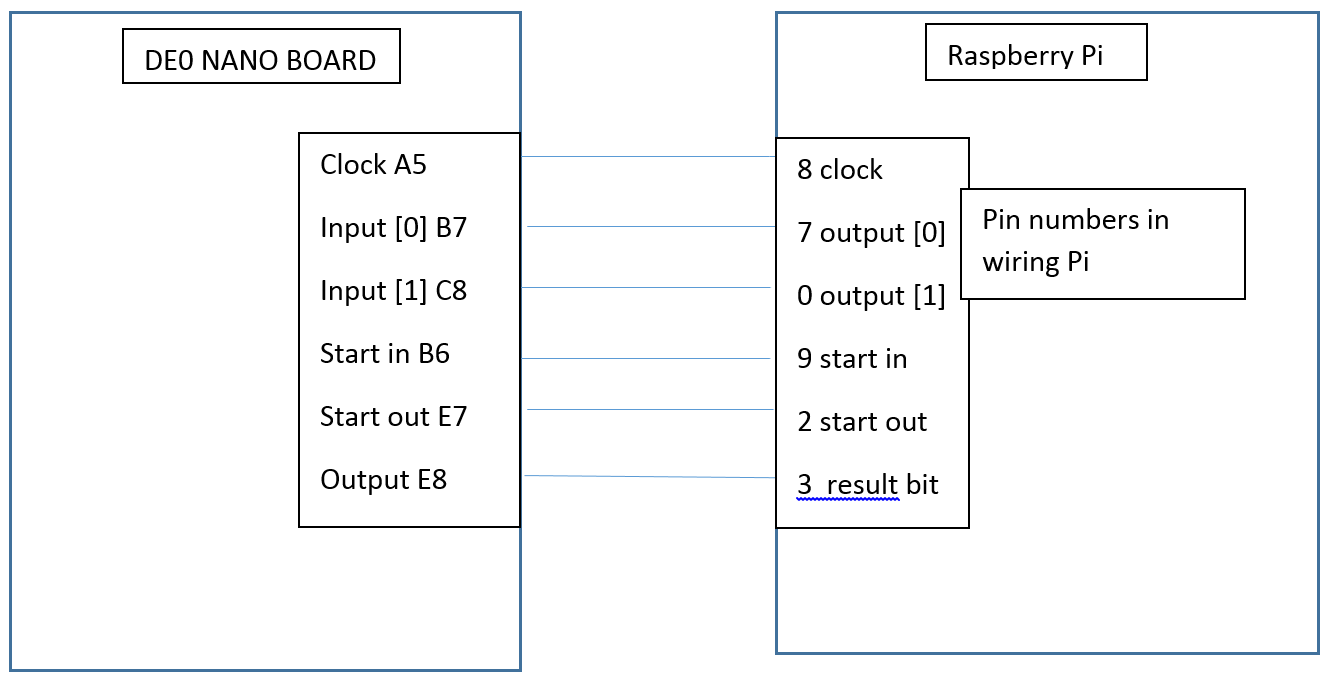
\includegraphics[scale=0.4]{./figs/DeNano_rPi}
  \caption{Block Schematic of DE0-Nano and Raspberry Pi interfacing}
  \label{DE0Nano_RPI}
\end{figure}


This system implementation works fine for frequency of 50 MHz maximum available frequency on DE0 Nano board i.e. gives result in 20nseconds but after interfacing with Raspberry Pi it takes total real time of 0.161sec much more compared to Ubuntu at 4th gen i-5 processor 0.005sec. The time needed for the Hardware / software implementation is greater due to the large data transfer at a lower clock rates limited by physical connections and 50MHz on-board clock. The performance can be improved with better interfacing and higher clock.

\textit{I would like to specially thank Siddharth and Abhinav, summer interns 2015, IIT Bombay, for the implementation of the above Bezier interpolation application implementation. And allowing me to use the results here}

\section{Raspberry Pi - FPGA for JTAG interface}


Raspberry Pi is very powerful ARM based CPU and a very convenient platform for adding additional interfaces to your hardware. For our board "Krypton v1.2", which is a CPLD/FPGA platform, we have FTDI serial cables, on-board USB port, a few other peripherals like LEDs, Switches etc..  and some GPIO port pins. This lets us flash and debug our hardware, communicate with it over serial (forwarded over a socket), and continuously monitor power consumption of key components on our board. And we can do it from anywhere with an internet connection. This helps us get remote access to the complete system allowing to update or completely change the HDL design without having a the platform in close proximity. The step to use Raspberry Pi as a JTAG programmer/Debugger these are some pre-requisites: 

\begin{enumerate}
\item{Acquire a R-Pi:}\\
First you’ll need a Raspberry Pi and an SD card with the Raspbian installed on it. You can get a Raspberry Model B Starter Kit from Newark. This comes with a power adapter and an SD card with NOOBS (which can automatically install Raspbian for you) pre-installed and is probably the easiest way to get started or a easy guide is available on Raspberry Pi wikipedia page.
\item{Install a Recent Version of OpeNoCD and urJTAG:}\\
There is a version of OpeNoCD already in the package database for Raspbian, but it’s version 0.6.1, which was too old for our platform. Fortunately it’s quite easy to install the latest OpeNoCD from scratch. There are pretty good instructions on how to do this at SourceForge. But specifically for the Pi you can just do the following:\\

\noindent From your Pi see the following command :

\begin{lstlisting}[language=bash]
pi>  sudo apt-get update
pi>  sudo apt-get install libtool libusb-dev libusb-1.0 autoconf automake texinfo
pi>  git clone git://git.code.sf.net/p/opeNoCd/code opeNoCd-code
pi>  cd opeNoCd-code/
pi>  ./bootstrap
pi>  ./configure
pi>  git clone git://git.code.sf.net/p/urjtag/git urjtag-git
pi>  cd urjtag-git
\end{lstlisting}

Edit the file cmd\_bfin.c in src/cmd and add the following line at the top:

\begin{lstlisting}[language=C]
#define _SYS_UCONTEXT_H
\end{lstlisting}
This is to avoid conflict between blackfin defines and system includes.

\begin{lstlisting}[language=bash]
pi>  ./autogen.sh
pi>  make
pi>  make install
pi>  sudo jtag

jtag> cable ft2232
jtag> detect
\end{lstlisting}

\end{enumerate}
This shall install all the necessary software tools needed for Raspberry Pi to work as a JTAG programmer/debugger tool. Detect command will detect the connected FPGA device. Refer Krypton manual \cite{kryptonManual} for more details on usage of urJTAG. 

\section{Motivation and Future Scope of using Raspberry Pi-FPGA Platform}
Raspberry Pi is very power full board developed for solving simple and complex problems. Developing a full flow of so that Raspberry Pi and FPGA can be utilized to their advantages will be of great significance. One such similar platform \cite{LOGIPi} built specifically for Raspberry Pi gives a great starting point. Taking one step further we can use Raspberry Pi for multiple FPGA device configuration. This architecture can be used for dynamic configuration of FPGA with different hardware designs along with software support provided by Raspberry Pi. In the next chapter we shall summarize this thesis work and also discuss future scope of the this project work. The chapter also show designs that can be implemented using the components discussed in this thesis.